
\documentclass[a4paper,12pt]{article}
\usepackage[margin=1in]{geometry}

\usepackage[T2A]{fontenc}			% кодировка
\usepackage[utf8]{inputenc}			% кодировка исходного текста
\usepackage[english,russian]{babel}	% локализация и переносы
\usepackage{graphicx}                % Математика
\usepackage{amsmath,amsfonts,amssymb,amsthm,mathtools} 
\usepackage{mathtext}
\usepackage[T2A]{fontenc}
\usepackage[utf8]{inputenc}

\usepackage{wasysym}

%Заговолок
\author{Бичина Марина 
группа Б04-005 1 курса ФЭФМ}
\title{Отчет по лабораторной работе №2.1.3


Определение $C_p/C_v$ по скорости звука в газе}
\date{12.03.2021}


\begin{document} % начало документа

\maketitle
\newpage

\section{Аннотация}

\paragraph{Цель работы:} 
\begin{enumerate}
\itemsep0em
\item ) Измерить частоту колебаний и длину волны при резонансе звуковых колебаний в газе, заполняющем трубу 
\item Определить показатель адиабаты с помощью уравнения состояния идеального газа.
\end{enumerate}
\paragraph{Оборудование:}
\begin{enumerate}
\itemsep0em
\item звуковой генератор ГЗ
\item электронный
осциллограф ЭО
\item микрофон
\item телефон
\item раздвижная труба
\item теплоизолированная труба, обогреваемая водой из термостата;
\item баллон со сжатым углекислым газом
\item газгольдер
\end{enumerate}
\section{Теоретическая часть}
\paragraph{} 
Скорость распространения звуковой волны в газах можно выразить формулой:
\begin{equation}
c = \sqrt{\gamma\frac{RT}{\mu}}
\end{equation}
где R - универсальная газовая постоянная, Т - температура газа, $\mu$ - молярная масса газа.

Отсюда можно выразить постоянную адиабаты, из формулы (1) равную:
\begin{equation}
\gamma = \frac{\mu}{RT}c^2
\end{equation}

Звуковая волна, распространяющаяся вдоль трубы, испытывает многократные отражения от торцов. Звуковые колебания в трубе являются наложением всех отраженных волн и, вообще говоря, очень сложны. Картина упрощается, если длина трубы L равна целому числу полуволн, то есть когда
\begin{equation}
L=n\frac{\lambda}{2}
\end{equation}
где $\lambda$ — длина волны звука в трубе, а $n$ — любое целое число.
		
Скорость звука c связана с его частотой $f$ и длиной волны $\lambda$ соотношением:
\begin{equation}
c=\lambda f
\end{equation}
		
Подбор условий, при которых возникает резонанс, можно производить двумя способами:
\begin{enumerate}
\itemsep0em
\item При неизменной частоте f звукового генератора (а следовательно, и неизменной длине звуковой волны $\lambda$) можно изменять длину трубы $L$. Для этого применяется раздвижная труба. Длина раздвижной трубы постепенно увеличивается, и наблюдается ряд последовательных резонансов. Для $k$-ого резонанса имеем:
\begin{equation}
		L_{n+k}=n\frac{\lambda}{2} + \frac{\lambda}{2},	
\end{equation}
т. е. $\lambda/2$ равна угловому коэффициенту графика, изображающего зависимость длины трубы $L$ от номера резонанса $k$.
\item При постоянной длине трубы можно изменять частоту звуковых колебаний. В этом случае следует плавно изменять частоту $f$ звукового генератора, а следовательно, и длину звуковой волны $\lambda$.
Для $k$-ого резонанса получим:
$$L = (n+k)\frac{\lambda_{k+1}}{2}$$
$$f_{k+1} = \frac{c}{\lambda_{k+1}}=\frac{c}{2L}(n+k)=f_1 + \frac{c}{2L}k.$$
		
Скорость звука таким образом по угловому коэффициенту графика зависимости частоты от номера резонанса.

\end{enumerate}
\subsection{Описание установки:}
\paragraph{}
Для двух методов измерения скорости звука в работе имеются две установки (рис. 1 и 2). В обоих случаях  они возбуждаются телефоном Т и улавливаются микрофоном М. Мембрана телефона приводится в движение переменным током звуковой частоты. В качестве источника переменной ЭДС используется звуковой генератор ГЗ. Возникающий в микрофоне сигнал наблюдается на осциллографе ЭО.

	Микрофон и телефон присоединены к установке через тонкие резиновые трубки. Такая связь достаточна для возбуждения и обнаружения звуковых колебаний в трубе и в то же время мало возмущает эти колебания: при расчетах оба торца трубы можно считать неподвижными, а влиянием соединительных отверстий пренебречь.



\begin{figure}[h]
\begin{center}
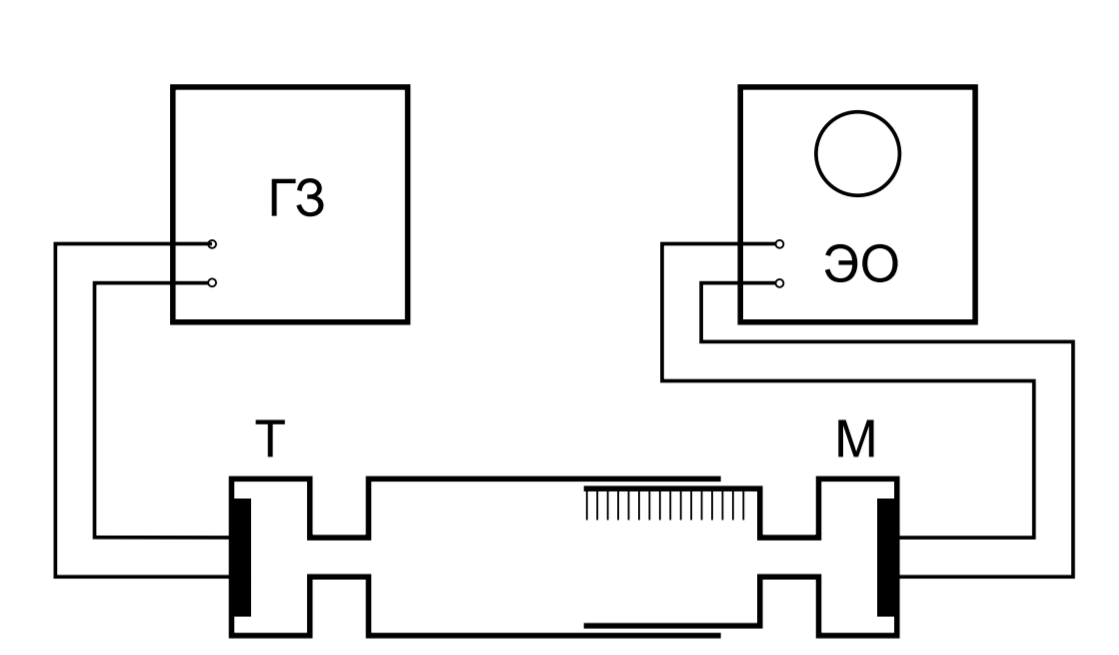
\includegraphics[width=0.6\linewidth]{ustanovka_1.png}
\caption{Установка для измерения скорости звука при помощи раздвижной трубы}
\label{ris:ustanovka_1} 
\end{center}
\end{figure}

	Первая установка (рис. 1) содержит раздвижную трубу с миллиметровой шкалой. Через патрубок (на рисунке не показан) труба может наполняться воздухом или углекислым газом из газгольдера. На этой установке производятся измерения $\gamma$ для воздуха и для $CO_2$


\begin{figure}[h]
\begin{center}
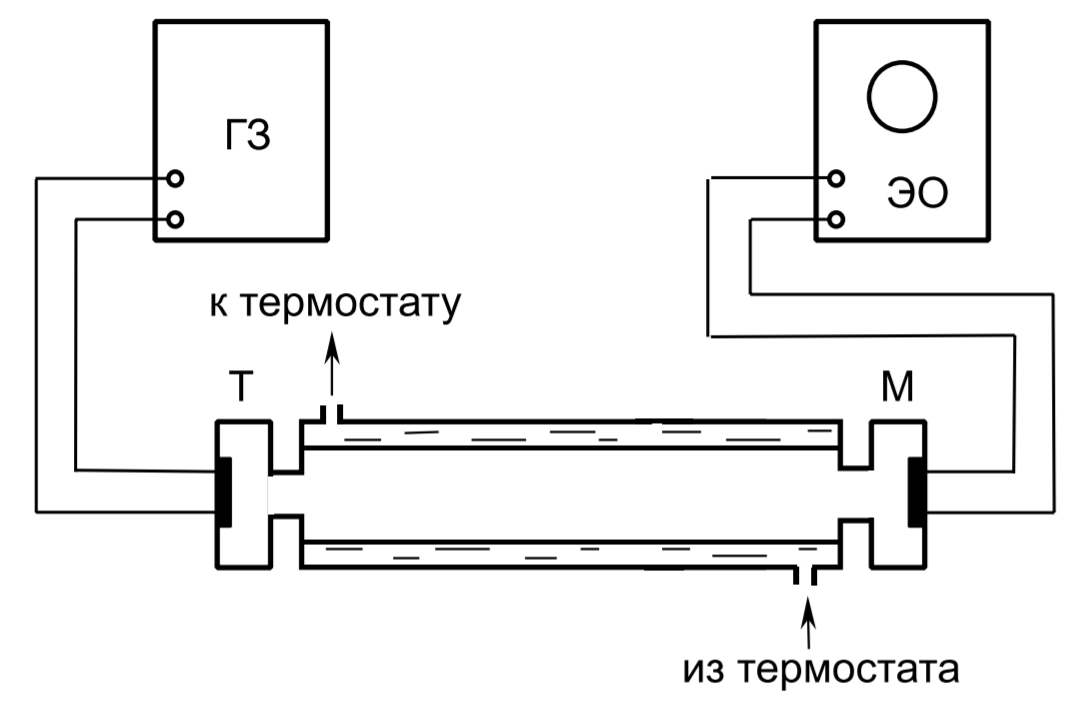
\includegraphics[width=0.6\linewidth]{ustanovka_2.png}
\caption{Установка для изучения зависимости скорости звука от температуры}
\label{ris:ustanovka_2} 
\end{center}
\end{figure}

Вторая установка (рис. 2) содержит теплоизолированную трубу постоянной длины. Воздух в трубе нагревается водой из термостата. Температура газа принимается равной температуре омывающей трубу воды. На этой установке измеряется зависимость скорости звука от температуры.


\subsection{Контрольные вопросы:}
\begin{enumerate}
\itemsep0em
\item Выведите формулы (1.16).\\

Из соотношения:
\[
c = \sqrt{\frac{E}{\rho}},
\]
Выразим модуль Юнга Е. Возьмем уравнения
\[
\Delta P = - E\frac{\Delta V}{V}, \;\;\;\;\ \frac{dV}{V} = - \frac{d\rho}{\rho}
\]

Отсюда получим: 

\[
E = \rho \frac{dP}{d\rho}.
\]
Подставляя в 1 получаем формулу (1.16):
\[
c = \sqrt{\frac{dP}{d\rho}}.
\]

\item Зависит ли $\gamma$ от температуры в выбранном интервале температур?\\

Нет, не зависит. $\gamma$ изменяется за счёт появления колебательный степеней свободы при высоких температурах, но в данном диапазоне это явление не происходит.

\item Будет ли наблюдаться такая зависимость при изменении температуры от очень малых значений до 1000 $^0C$?\\

 При температурах около 1000 $ ^0C$ будут вносить вклад колебательные степени свободы и $\gamma$ будет изменяться.
\end{enumerate}
\section{Ход работы:}
\begin{enumerate}
\renewcommand{\labelenumii}{\arabic{enumii})}
\itemsep0em
\item Включим в сеть электронный осциллограф ЭО и звуковой генератор ГЗ, дадим им прогреться 5-7 минут. После этого включим тумблер <<Луч>> и добьемся, чтобы на экране была видна линия, прочерченная электронным лучом.

	Установим нулевое значение шкалы частот звукового генератора.
\item Подберем напряжение на выходе генератора так, чтобы при резонансе на осциллографе наблюдались колебания достаточной амплитуды.

Остановим картину на осциллографе. Убедимся в том, что колебания имеют неискаженную синусоидальную форму.
\item Измерения на первой
установке (рис. 1).

\begin{enumerate}
\itemsep0em
\item Исходя из примерного значения скорости звука (300 м/с), рассчитаем, в каком диапазоне частот следует вести измерения, чтобы при удлинении трубы можно было наблюдать 2–5 резонансов
\item Используя многоходовый или кнопочный кран, продуем трубу воздухом(в ней мог остаться углекислый газ).Повторим измерения при других частотах (всего 4–6 различных значений частоты). Для каждого резонанса измерим соответствующее удлинение трубы. Проведем измерения, сначала увеличивая длину трубы, а затем уменьшая ее. Результаты сведем в таблицу 1 
\begin{table}[h]
\begin{center}
\begin{tabular}{|c|c|c|c|c|c|}
\hline 
$f$, Гц & $1$ & $2$ & $3$ & $4$ & $5$ \\ 
\hline 
$ 719 $ & $ \uparrow 46 , \; \downarrow 47 $ & -- & -- & -- & -- \\ 
\hline 
$ 1398 $ & $ \uparrow 25 , \; \downarrow 22 $ & $ \uparrow 146 , \; \downarrow 150 $ & -- & -- & -- \\ 
\hline 
$ 2095 $ & $ \uparrow 40 , \; \downarrow 41 $ & $ \uparrow 123 , \; \downarrow 122 $ & $ \uparrow 205 , \; \downarrow 206 $ & -- & -- \\ 
\hline 
$ 2793 $ & $ \uparrow 48 , \; \downarrow 47 $ & $ \uparrow 109 , \; \downarrow 110 $ & $ \uparrow 171 , \; \downarrow 171 $ & -- & -- \\ 
\hline 
$ 3500 $ & $ \uparrow 42 , \; \downarrow 43 $ & $ \uparrow 92 , \; \downarrow 93 $ & $ \uparrow 142 , \; \downarrow 143 $ & $ \uparrow 191 , \; \downarrow 191 $ & -- \\ 
\hline 
$ 4206 $ & $ \uparrow 41 , \; \downarrow 41 $ & $ \uparrow 82 , \; \downarrow 83 $ & $ \uparrow 125 , \; \downarrow 124 $ & $ \uparrow 165 , \; \downarrow 165 $ & $ \uparrow 206 , \; \downarrow 206 $ \\ 
\hline 
\end{tabular} 
\end{center}
\caption{Данные полученные для воздуха}
\label{air}
\end{table}
\item Изобразим полученные результаты на графике, откладывая по оси абсцисс номер
$k$ последовательного резонанса, а по оси ординат — соответствующее удлинение трубы $L_{(n+k)}-L_n$. Через точки, полученные при одном и том же значении частоты, проведем наилучшую прямую по мнк. Угловой коэффициент прямой определяет длину полуволны.
По графику оценим ошибку измерения $\lambda/2$. Вычислим значение
скорости звука
и оценим точность полученного результата. Найдем наилучшее значение скорости звука, используя все результаты измерений

\paragraph{} По измеренным данным построим графики зависимости длины трубы $L$ от номера резонанса $N$. И проведём наилучшею прямую по методу наименьших квадратов:

\begin{equation}
b = \frac{\langle xy \rangle - \langle x \rangle \langle y \rangle}{\langle x^2 \rangle - \langle x \rangle ^ 2}, \;\;
a = \langle y \rangle - b \langle x \rangle . \label{lsf}
\end{equation}
\begin{equation}
\sigma_b \approx \frac{1}{\sqrt{N}}\sqrt{\frac{\langle y^2 \rangle - \langle y \rangle ^ 2}{\langle x^2 \rangle - \langle x \rangle ^ 2} - b^2}, \;\;
\sigma_a = \sigma_b \sqrt{\langle x^2 \rangle - \langle x \rangle ^ 2}. \label{lsfvar}
\end{equation}

Для наших целей значение $a$ не требуется, получим формулы:
\begin{equation}
\lambda/2 = \frac{\langle NL \rangle - \langle N \rangle \langle L \rangle}{\langle N^2 \rangle - \langle N \rangle ^ 2}, \;\;
\sigma_{\lambda} \approx \frac{1}{\sqrt{n}}\sqrt{\frac{\langle L^2 \rangle - \langle L \rangle ^ 2}{\langle N^2 \rangle - \langle N \rangle ^ 2} - \left(\lambda/2\right)^2} . \label{lsf2}
\end{equation}

Подставив значения из таблицы \ref{air} в форумы получим значения для воздуха:


\begin{center}
\begin{tabular}{|c|c|c|c|c|c|}
\hline 
$f$ & 1398 & 2095 & 2793 & 3500 & 4206 \\ 
\hline 
$\langle N \rangle$ & 1.5 & 2.0 & 2.0 & 2.5 & 3.0 \\ 
\hline 
$\langle L \rangle$ & 85.75 & 122.83 & 109.33 & 117.13 & 123.8 \\ 
\hline 
$\langle NL \rangle$ & 159.75 & 300.67 & 259.83 & 354.75 & 453.9 \\ 
\hline 
$\langle N^2 \rangle$ & 2.5 & 4.67 & 4.67 & 7.5 & 11.0 \\ 
\hline 
$\langle L^2 \rangle$ & 11231.25 & 19625.83 & 14496.0 & 16787.63 & 18729.8 \\ 
\hline 
$\lambda/2$ & 124.5 & 82.5 & 61.8 & 49.6 & 41.3 \\ 
\hline 
$\sigma_{\lambda/2}$ & 1.8 & 0.3 & 0.2 & 0.2 & 0.2 \\ 
\hline 
\end{tabular} 
\end{center}


\item Измерим скорость звука в углекислом газе. Перед началом измерений продуем трубу углекислым газом. По окончании этих измерений подвижную часть трубы оставим во вставленном состоянии и провем измерения резонансных максимумов при увеличении и затем при уменьшении частоты. Сведем данные в таблицу 2. Обработаем полученные данные и сравним результаты с полученными при изменении длины трубы
\begin{table}[h]
\begin{small}
\begin{center}
\begin{tabular}{|c|c|c|c|c|c|c|}
\hline 
$f$, Гц & $1$ & $2$ & $3$ & $4$ & $5$ & $6$ \\ 
\hline 
$702$ & $ \uparrow 27 , \; \downarrow 28 $ & $ \uparrow 218 , \; \downarrow 217 $ & -- & -- & -- & -- \\ 
\hline 
$1405$ & $ \uparrow 80 , \; \downarrow 81 $ & $ \uparrow 178 , \; \downarrow 176 $ & -- & -- & -- & -- \\ 
\hline 
$2099$ & $ \uparrow 6 , \; \downarrow 6 $ & $ \uparrow 70 , \; \downarrow 70 $ & $ \uparrow 135 , \; \downarrow 134 $ & $ \uparrow 198 , \; \downarrow 199 $ & -- & -- \\ 
\hline 
$2799$ & $ \uparrow 21 , \; \downarrow 21 $ & $ \uparrow 69 , \; \downarrow 69 $ & $ \uparrow 117 , \; \downarrow 117 $ & $ \uparrow 165 , \; \downarrow 165 $ & $ \uparrow 213 , \; \downarrow 214 $ & -- \\ 
\hline 
$3495$ & $ \uparrow 32 , \; \downarrow 32 $ & $ \uparrow 72 , \; \downarrow 70 $ & $ \uparrow 108 , \; \downarrow 108 $ & $ \uparrow 147 , \; \downarrow 147 $ & $ \uparrow 190 , \; \downarrow 185 $ & $ \uparrow 226 , \; \downarrow 225 $ \\ 
\hline 
\end{tabular} 
\end{center}
\end{small}
\caption{Данные полученные для CO$_2$}
\label{co2}
\end{table}
\end{enumerate}
\paragraph{} Аналогично воздуху, построим график для углекислого газа по методу мнк, применяя формулу \ref{lsf}, опираясь на значения таблицы \ref{co2}

\begin{center}
\begin{tabular}{|c|c|c|c|c|c|}
\hline 
$f$ & 702 & 1405 & 2099 & 2799 & 3495 \\ 
\hline 
$\langle N \rangle$ & 1.5 & 1.5 & 2.5 & 3.0 & 3.5 \\ 
\hline 
$\langle L \rangle$ & 122.5 & 128.75 & 102.25 & 117.1 & 128.5 \\ 
\hline 
$\langle NL \rangle$ & 231.25 & 217.25 & 335.88 & 447.5 & 562.75 \\ 
\hline 
$\langle N^2 \rangle$ & 2.5 & 4.67 & 7.5 & 11.0 &  15.17 \\ 
\hline 
$\langle L^2 \rangle$ & 24031.5 & 18905.25 & 15607.25 & 18339.7 & 20892.0 \\ 
\hline 
$\lambda/2$ & 190.0 & 96.5 & 64.2 & 48.1 & 38.7 \\ 
\hline 
$\sigma_{\lambda/2}$ & 0.5 & 0.8 & 0.2 & 0.1 & 0.3 \\ 
\hline 
\end{tabular} 
\end{center}
\item Вычислим значение $\gamma =C_p/C_v$ по формуле (1). Оценим ошибку измерений.

Найдём по полученным из графиков значениям скорость звука по формулам:

\begin{equation}
c = f \lambda, \;\;\; \sigma_c = c \sqrt{(\sigma_f/f)^2 + (\sigma_\lambda/\lambda)^2},
\label{speed}
\end{equation}

\noindent где $f$ -- частота, $\lambda$ -- длина волны, $\sigma_f = 1 \; \text{Гц}, \; \sigma_{\lambda} = 2 \sigma_{\lambda/2`}$.

Подставив в (\ref{speed}) значения для воздуха получим:
\begin{center}
\begin{tabular}{|c|c|c|c|c|c|}
\hline
$ f $ & 1398 & 2095 & 2794 & 3501 & 4206 \\
\hline
$ \lambda$ & 249.0 & 165.0 & 123.4 & 99.2 & 82.4 \\
\hline
$ \sigma_{\lambda}$ & 3.6 & 0.6 & 0.4 & 0.4 & 0.2 \\
\hline
$ c $ & 348.0 & 346.0 & 345.0 & 347.0 & 347.0 \\
\hline
$ \sigma_c $ & 6.0 & 2.0 & 2.0 & 2.0 & 1.0 \\
\hline
\end{tabular}
\end{center}

Подставив в (\ref{speed}) значения для углекислого газа получаем:
\begin{center}
\begin{tabular}{|c|c|c|c|c|c|}
\hline
$ f $ & 702 & 1405 & 2099 & 2799 & 3495 \\
\hline
$ \lambda$ & 380.0 & 193.0 & 128.4 & 96.2 & 77.4 \\
\hline
$ \sigma_{\lambda}$ & 1.0 & 1.6 & 0.2 & 0.2 & 0.4 \\
\hline
$ c $ & 267.0 & 271.0 & 270.0 & 269.0 & 271.0 \\
\hline
$ \sigma_c $ & 1.0 & 3.0 & 1.0 & 1.0 & 2.0 \\
\hline
\end{tabular}
\end{center}

Далее вычислим $\gamma = C_p / C_v $ по формуле (\ref{gamma}) подставив полученные значения для $c$ и $\mu_{возд.} = 0.02897$ кг/моль, $ \mu_{\text{CO}_2} = 0.044 $ кг/моль:

\[
\gamma_{возд.} = \frac{\mu_{возд.}}{RT} c^2_{\text{возд.}}, \;\;\; \gamma_{\text{CO}_2} = \frac{\mu_{\text{CO}_2}}{RT} c^2_{\text{CO}_2}, \;\;\; \sigma_{\gamma} = \gamma \sqrt{4 \left(\frac{\sigma_c}{c} \right)^2 + \left(\frac{\sigma_T}{T} \right)^2}.
\]

\noindent Исходя из данных в таблицах возьмём $c_{\text{возд.}} = 346 \pm 2$ м/с,  $c_{\text{возд.}} = 270 \pm 2$ м/с, температура воздуха $T = 297 \pm 2$ К:

\[
\gamma_{\text{возд.}} = \frac{0.02897}{8.314 \cdot 297} \cdot 346^2 \approx 1.40 ,\;\;\;
\sigma_{\gamma_\text{возд.}} = 1.40 \cdot \sqrt{4 \left(\frac{2}{346} \right)^2 + \left(\frac{2}{297} \right)^2} \approx 0.02  ;
\]
\[
\gamma_{\text{CO}_2} = \frac{0.044}{8.314 \cdot 297} \cdot 270^2 \approx 1.30 ,\;\;\;
\sigma_{\gamma_{\text{CO}_2}} = 1.30 \cdot \sqrt{4 \left(\frac{2}{270} \right)^2 + \left(\frac{2}{297} \right)^2} \approx 0.03 .
\]

Полученные нами значения для показателей адиабаты: $ \gamma_{\text{возд.}} = 1.40 \pm 0.02, \; \gamma_{\text{CO}_2} = 1.30 \pm 0.03 $.
\end{enumerate}
\section{Выводы:}
\begin{enumerate}
\item
Установили линейную зависимость длины трубы от номера резонанса 
\item
Измерили скорость звука в воздухе и углекислом газе при комнатной температуре.

$c_{\text{возд}} = 346 \pm 2$ м$/$c ($\varepsilon_c = 0.6 \% $), $c_{\text{CO}_2} = 270 \pm 2$ м$/$с ($ \varepsilon_c = 0.7 \% $).

\item
Вычисли показатель $\gamma = C_p/C_v$ для воздуха и углекислого газа при комнатной температуре:

 $\gamma_{\text{возд}} = 1.40 \pm 0.02 \; (\varepsilon_\gamma = 1.5 \%), \; \gamma_{\text{CO}_2} = 1.30 \pm 0.03 \; (\varepsilon_\gamma = 2.4 \%)$.

\end{enumerate}
\end{document}